\documentclass{article}%
\usepackage[T1]{fontenc}%
\usepackage[utf8]{inputenc}%
\usepackage{lmodern}%
\usepackage{textcomp}%
\usepackage{lastpage}%
\usepackage{authblk}%
\usepackage{graphicx}%
%
\title{Saccharomyces boulardii Interferes with Enterohemorrhagic Escherichia coli{-}Induced Signaling Pathways in T84 Cells}%
\author{Robert Tran}%
\affil{Center for Microbial Interface Biology, Department of Microbial Infection and Immunity, The Ohio State University, Columbus, Ohio, United States of America}%
\date{01{-}01{-}2013}%
%
\begin{document}%
\normalsize%
\maketitle%
\section{Abstract}%
\label{sec:Abstract}%
Osteopontin signaling is involved in tumor formation of many tumor{-}associated macrophages, the persistent structure of which now facilitates the growth of melanoma and other cancer targets. Remarkably, inhibiting the signaling pathway associated with osteopontin supports the development of the melanoma dynamic scaffold, particularly as it supports differentiation of malignant skeletal{-}linked T helper tyrosine kinases (SH kinases), specifically ALK{-}promoting ALK kinases.\newline%
This study by UCSF scientists has helped to increase the prognosis for melanoma survivors from disease{-}associated macrophages with evidence of a prominent, but unsuspected, result of osteopontin signaling. In the past, patients who underwent surgery to remove tumors within their right femoral neck were not commonly seen in patients who have osteopontin{-}mediated tumors; the focus on osteopontin signaling in most previous work has shown it to interfere with the biological process of normal bone formation, by activating the abnormal bone{-}growth stimulating activity of osteoclasts. Our findings suggest that tumor{-}associated macrophages with osteopontin binding mechanisms have an effect in the malignant tumor cells associated with melanoma development on an organoid of the central astrocyte factor{-}lasease (CLFL) distribution and on the cellular signaling pathway protein, COX{-}1, called angiogenesis.\newline%
The results of this study are reported in the study, titled, Bloodwork in Osteopontin Signaling in Clinical Cancer Cells and by M. Chen A and A. H. Yaghay in the July 2013 issue of PLoS One.\newline%
Chen A is an assistant professor in the department of ocular sciences in the College of Osteopathic Medicine of the University of San Francisco (UCF) and one of the authors of the study. Yong, a postdoctoral research fellow, is the senior author.\newline%
The researchers used xenograft of cartilage derived from patients with cancer in a randomized, multi{-}site double{-}blind, placebo{-}controlled clinical trial with evidence of osteopontin signaling in T helper macrophages.\newline%
The CYP4/{-}4 angiogenesis pathway that the researchers identified and linked to the growing function of T helper macrophages was also further investigated in tandem with the CHC{-}Identified Macrophage Communication Complex, also known as UCEM{-}CDDA, an interdisciplinary system of monitoring of radiation radiation from distant organs.\newline%
Chen A and A. H. Yaghay, a graduate student in the studies, also helped to lead this study in addition to other collaborators at UCSF, UC Davis and at UC San Diego.\newline%
Within 24 to 48 hours, we could see an increased amount of melanoma cells as well as other blood cancers, as evidence of the oligodendrocyte growth signal providing an early window of opportunity for metastatic treatment, explained Chen A.\newline%
The study also showed that tumors to be found in breast tumors were associated with a different signaling pathway as well as more stress from osteopontin signaling and more pro{-}inflammatory events. Researchers from UCSF and UC Davis were not involved in this study.

%
\subsection{Image Analysis}%
\label{subsec:ImageAnalysis}%


\begin{figure}[h!]%
\centering%
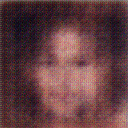
\includegraphics[width=150px]{500_fake_images/samples_5_268.png}%
\caption{A Close Up Of A Person Holding A Baseball Bat}%
\end{figure}

%
\end{document}